\chapter{Vorbereitung}
\section{Der Operationsverstärker}
\subsection{Allgemeines}

\begin{figure}[H]
     \centering
     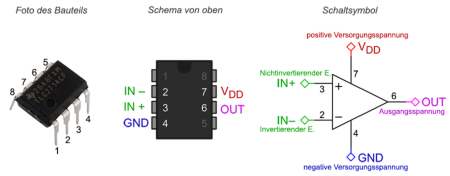
\includegraphics[width=1\textwidth]{Abb/opamp.pdf}
     \caption{Der Operationsverstärker}
     \label{opamp}
\end{figure}
OPV besitzen i. A. fünf entscheidende Ein- und Ausgänge. Einen sog. invertierenden Eingang (-), einen sog. nicht invertierenden Eingang (+), einen Ausgang und Anschlüsse für die Versorgungsspannung.
OPV können sehr hohe Spannungsverstärkungen ($10^{5}$ bis $10^{6}$), sehr hohe Eingangsimpedanzen ($108 \Omega$) und sehr geringe Ausgangsimpedanzen ($20 \Omega$) besitzen. 
Der OPV kann als invertierender oder als nicht invertierender Verstärker verwendet werden. Beide modulieren das eingehende Signal.

\subsection{Invertierender Verstärker}

\begin{figure}[H]
    \centering 
    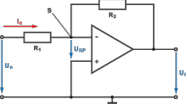
\includegraphics[width=0.7\textwidth]{Abb/invamp.pdf}
    \caption{Das Schaltbild eines invertierenden Verstärkers mit OPV}
    \label{inv}
\end{figure}
Abb. \ref{inv} zeigt das Schaltbild eines invertierenden Verstärkers mit OPV. Da (+) auf Masse liegt, stellt sich dies als Potential für (-) ein; man spricht von einem virtuellen Massepunkt. Daraus folgt, dass über R2 die Spannung Ua und über R1 die Spannung Ue abfällt. Über die Eingänge fließt kein Strom, somit gilt $U_eR_1=-U_aR_2$. Für die Spannungsverstärkung heißt das:
$v= U_a/U_e =-R_2/R_1$

\subsection{Nichtinvertierender Verstärker}

\begin{figure}[H]
    \centering
    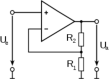
\includegraphics[width=0.5\textwidth]{Abb/ninv.pdf} 
    \caption{Schaltbild eines nichtinvertierenden Verstärkers}
    \label{ninv}
\end{figure}
In Abb. \ref{ninv} ist das Schaltbild eines nichtinvertierenden Verstärkers zu sehen. Da (+) auf Ue liegt, wird auch (-) auf dieses Potential gezwungen. Am Spannungsteiler gilt somit:
$U_e=U_a·R_1R_1+R_2$. 
Damit folgt für Spannungsverstärkung:
$v=U_a/U_e=1+R_2/R_1$

\subsection{Realer/idealer OPV}

Folgende Grafik beschreibt die entscheidenden Unterschiede zwischen dem idealen und dem realen Operationsverstärker.
Klar ist, dass wir im realen nie einen unendlich großen oder Null- Widerstand herstellen können. Der Ideale OPV ist weit entfernt vom Realen, doch die Tendenzen des Realen OPV gehen klar in die richtige Richtung. Bipolar und FET beschreiben, in dieser Tabelle, die Art der Transistoren, die im OPV verbaut wurden. Sie unterscheiden die Wirkung des OPV’s nur gering.

\begin{figure}[H]
     \centering
     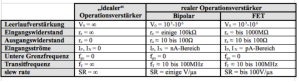
\includegraphics[width=0.9\textwidth]{Abb/vergl.pdf}
     \caption{Vergleich zwischen realem und idealem Operationsverstärker}
\end{figure}

\subsection{Impedanzwandler}

Der Impedanzwandler entspricht dem nicht-invertierendem Verstärker, mit einem Verstärkungsfaktor von 1. Im Schaltbild also ohne Spannungsteiler zu sehen. Man setzt also den Widerstand $R_1$ auf 0, damit die Formel $A= 1+ R_1/R_2 = 1$ ergibt.
\begin{figure}[H]
     \centering
     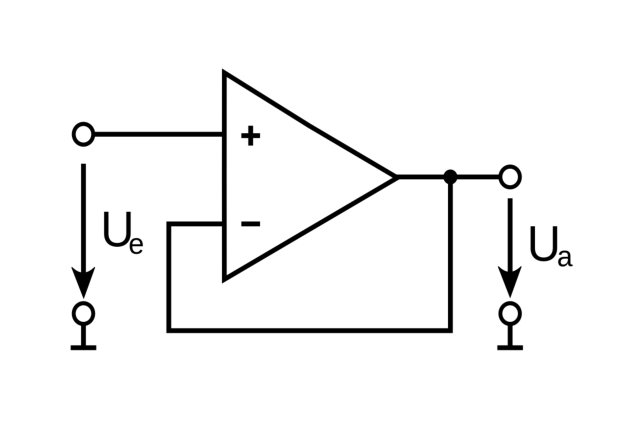
\includegraphics[width=0.7\textwidth]{Abb/impconv.pdf}
     \caption{Schaltbild eines Impedanzwandlers}
\end{figure}
Ein Impedanzwandler ist essenziell um Systeme mit verschieden großer Impedanz aneinander anzupassen. Also die geringe Stromstärke, die der menschliche Körper mit seinem Herzschlag erzeugt, auf eine verwertbare anzuheben, ohne dabei die Spannung zu verändern. Andernfalls wäre das Signal nicht in der Lage verschiedene Operationen ohne Veränderung zu überstehen (verschiedene Filter, Messausschläge bei Analogen Geräten). Er besitzt eine große Eingangsimpedanz und eine geringe Ausgangsimpedanz. 

\subsection{Analog-Digital-Wandler}

Ein A-D-Wandler setzt ein analoges Eingangssignal in digitale Daten um. Dazu wird in einer festgelegten Abtastfrequenz jedem Spannungswert eine Binärzahl zugeordnet.
Zu sehen in Abbildung \ref{adw} ist, welche Bedeutung die Anzahl der Bits auf den erhalt gut beschriebener Schwingungen hat. Dies wird auch als Auflösung bezeichnet. Die Anzahl der Bits wird auch Quantisierungszustände genannt.
\begin{figure}[H]
     \centering     
     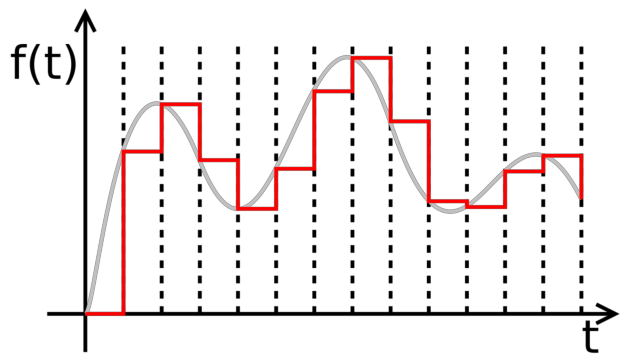
\includegraphics[width=0.7\textwidth]{Abb/adw.pdf}
     \caption{Wandlung eines analogen Signals in ein Digitales}
     \label{adw}
\end{figure}
Ein A-D-Wandler ist ideal ausgesteuert, wenn die maximal erreichte Eingangsspannung mit der höchstmöglichen Binärzahl kodiert wird. 
Nach dem sog. Nyquist-Shannon-Abtasttheorem muss die Abtastfrequenz mindestens doppelt so groß sein wie die maximal mögliche Eingangsfrequenz. Andernfalls spricht man von Unterabtastung, das sog. Aliasing. Dabei werden Frequenzen, die höher sind als die halbe Abtastfrequenz, als niedrigere Frequenzen interpretiert.
\begin{figure}[H]
    \centering
    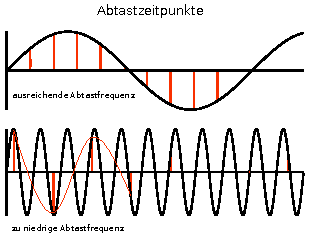
\includegraphics[width=0.6\textwidth]{Abb/abtast.pdf} 
    \caption{Effekt einer zu kleinen Abtastfrequenz: Nyquist-Shannon-Abtasttheorem}
\end{figure}

\subsection{Hoch- und Tiefpassschaltungen}
Die verwendeten Analogfilter setzen sich wie folgt zusammen.
(L, ohne Index, stünde hier für eine Spule, ist im generellen jedoch ein gewöhnlicher Widerstand.)
\begin{figure}[H]
    \centering
    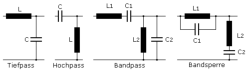
\includegraphics[width=\textwidth]{Abb/pass.pdf} 
    \caption{Schaltbilder verschiedener Frequenzfilter}
    \label{pass}
\end{figure}

\subsubsection{RC-Hochpass}
Abb. \ref{pass} zeigt das Schaltbild eines RC-Hochpasses erster Ordnung. Die Schaltung stellt einen Spannungsteiler mit Kondensator und Widerstand dar.
Als Grenzfrequenz $f_g$ bezeichnet man diejenige Frequenz, bei der $U_a$ gegenüber $U_e$ um drei Dezibel abgeschwächt ist, die Formel hierfür lautet: $f_g=1/2\pi R C$

\subsubsection{RC-Tiefpass}

In Abb. \ref{pass} ist das Schaltbild eines RC-Tiefpasses erster Ordnung zu sehen. Auch hier ergibt sich für die Grenzfrequenz: $f_g=1/2 \pi RC$
Er verändert ein Rechtecksignal wie folgt:

\subsubsection{Bandsperre}
Die Bandbreite einer Bandsperre ist die Größe des Frequenzbereichs zwischen oberer und unterer Grenzfrequenz, also $f_O -f_U$.
Unter der Mittenfrequenz einer Bandsperre versteht man das geometrische Mittel aus oberer und unterer Grenzfrequenz, also: $f_0=\sqrt{(f_O·f_U)}$
Die Güte beschreibt im Allgemeinen das Maß der Dämpfung in einem Schwingkreis, wie es diese Schaltungen sind.
Ist die Güte Groß, so ist die Dämpfung klein.
\begin{figure}[H]
    \centering
    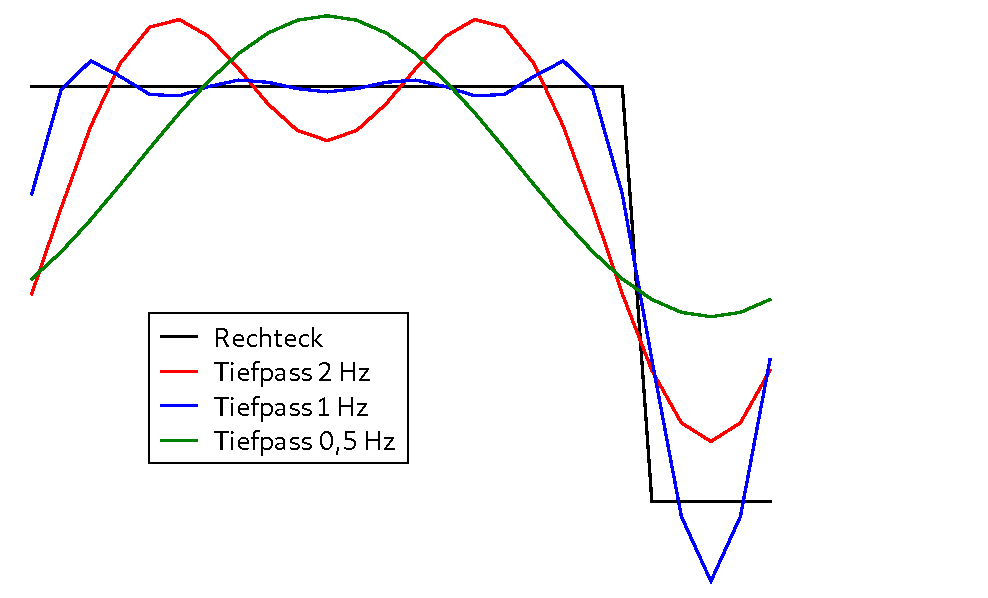
\includegraphics[width=0.6\textwidth]{Abb/rechtecktief.pdf} 
    \caption{Anwendung eines Tiefpass auf ein Rechtecksignal}
\end{figure}

\subsubsection{Bode-Diagramme}
Die Bode-Diagramme beschreiben zwei Arten von Graphen. Zum einen gibt es den Graph der Amplitudenverstärkung, zum anderen den Graphen der Phasenverschiebung. Sie tragen Amplitude/Phase gegen die Frequenz auf und kann damit charaktaristische Bauteile wie Filter und Pässe darstellen. Zu sehen in Abbildung 8 ist ein Beispiel der Bode-Diagramme zu einem Tiefpass. Es ist deutlich zu sehen, dass die Amplitude bei Hohen Frequenzen stark abnimmt, und bei der Grenzfrequenz die Phasenverschiebung am stärksten ist.
\begin{figure}[H]
    \centering
    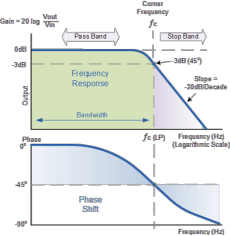
\includegraphics[width=0.6\textwidth]{Abb/bode.pdf}
    \caption{Bode-Diagramme} 
\end{figure}

Eine typische Größe zur Darstellung der Amplitude ist das Dezibel. Dieses wird für die Leistung wie folgt berechnet:
P(dB)=10lg(P/P0)
Wir verwenden einfach die Spannung, dies ist erlaubt, da P= U*I

\subsection{Fouriertransformation }
Die Fourier-Transformation erlaubt es ein Zeitsignal einer aperiodischen Funktion $f(x)$ in ein Spektrum $F(\omega)$ zu zerlegen. Dabei gibt $f(x)$ den Zeitbereich an und $F(\omega)$ den Frequenzbereich. Demnach kann angenommen werden, dass x = Zeit ist und $\omega= $Frequenz. 
Dabei unterscheidet man zwischen verschiedenen Typen. Graphisch sieht dies folgendermaßen aus:
\begin{figure}[H]
     \centering
     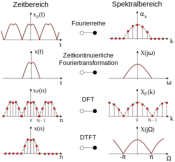
\includegraphics[width=0.6\textwidth]{Abb/fourier.pdf}
\end{figure}
Allgemein gilt: Je größer das Zeitfenster, desto größer die erzielbare Frequenzauflösung, aber desto kleiner ist die Zeitauflösung.

Eine weiterer Gewinn durch die Fouriertransformation ist das Digitale Filtern von Frequenzen. Die sog. Fast-Fourier-Transformation zerlegt ein Signal in sein Spektrum, entfernt störende Frequenzen und rücktransformiert das neue Signal. So lassen sich Digital in kurzer Zeit Signale deutlich „verschönern“.

\subsection{Technische Herausforderungen bei der Aufnahme von Elektrokardiogrammen}
Beim Messen von EKG-Signalen sind möglich durch:

Elektrische Streufelder:
  Abschrimung der Signalführenden Kabel und Verwendung von Filtern gegen störende Nebensignale.
Magnetische Streufelder:
  Kabel verdrillen, die Patientenlage ändert und erhöter Abstand zu Störquellen.
Messverstärker:
  Hohe Eingangsimpedanz, da auch unser Körper eine Hohe Impedanz besitzt. Unnötige Verkabelung vermeiden.
Elektroden:
  Kontaktspray verwenden, und die Klemmen fest am Körper befestigen, um Aussetzer des Signals zu vermeiden.
